\section{Case study}
Trong phần này chúng ta sẽ cùng theo dõi và phân tích một dashboard thực tế mà tác giả cùng đội của mình xây dựng để giám sát hệ thống OCR đọc thông tin từ giấy tờ của người dùng. Tính năng chính của hệ thống là nhận vào url ảnh giấy tờ (trên hệ thống lưu trữ tập trung của doanh nghiệp) và trích xuất thông tin. Những thông số quan trọng nhất trong ứng dụng kiểu này đó là tài nguyên hệ thống, thời gian xử lý và phản hồi của các hệ thống có kết nối đến. 

Dữ liệu giám sát phần cứng được Grafana giao tiếp với hệ điều hành, còn các dữ liệu do người lập trình tự định nghĩa được lưu trữ dưới dạng log ở Elasticsearch (sẽ được nói đến kĩ hơn ở phần sau của bài báo cáo).

\begin{figure}[H] % places figure environment here   
    \centering % Centers Graphic
    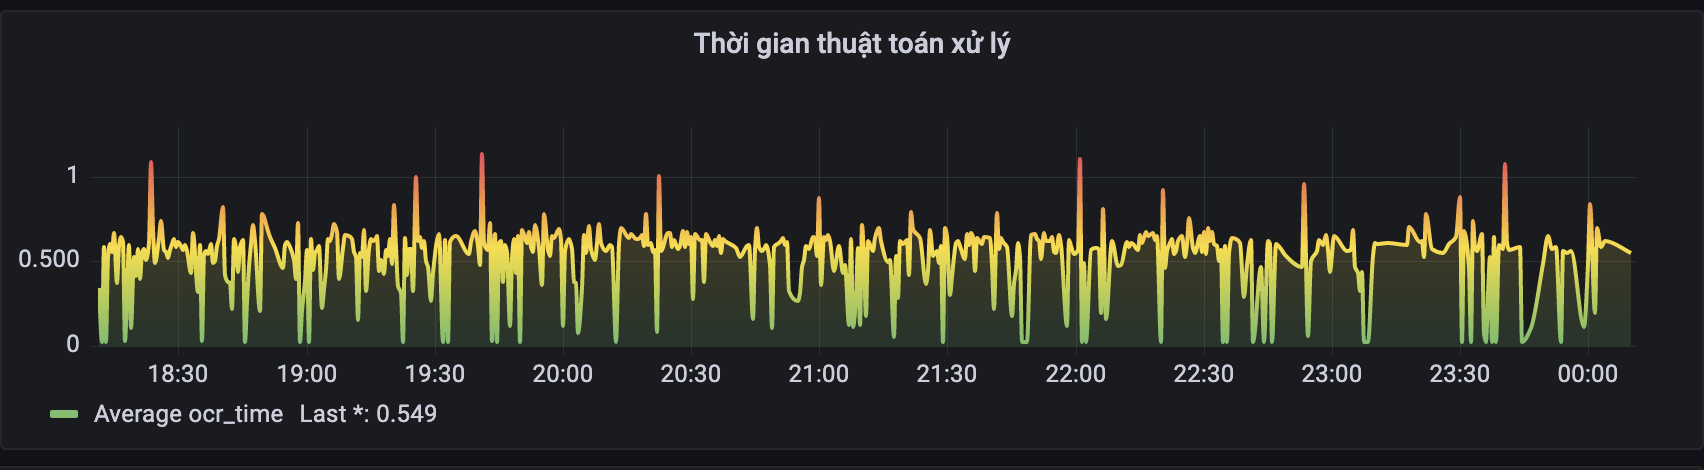
\includegraphics[width=1\textwidth]{figures/computing_time.png} 
    \caption{Thời gian ứng dụng trích xuất thông tin từ ảnh} % Creates caption underneath graph
    \label{fig:elk_01}
\end{figure}

Trên hình là biểu đồ theo thời gian của thời gian trung bình mà ứng dụng trích xuất kí tự từ ảnh. Biểu đồ đường được sử dụng kết hợp với lớp phủ màu. Thời gian xử lý chuyển từ sắc xanh, vàng sang cam, đỏ. Lớp phủ màu được thêm vào để tiện cho người dùng quan sát tổng quan, càng nhiều màu đỏ nghĩa là thời gian tính toán càng lâu, ngược lại, khi màu xanh chiếm đa số có nghĩa là ứng dụng đang tính toán nhanh. Trong khoảng thời gian được cắt ra trên hình ta có thể nhận thấy thời gian tính toán trung bình vào khoảng 0.5s và thời gian xử lý lâu nhất vào khoảng 1s. Điều này đang được chấp nhận trong thực tế do tài nguyên phần cứng của ứng dụng OCR này đang được dùng chung cho nhiều ứng dụng khác nữa. Hiện đội đang sử dụng GPU là Tesla T4 khá cũ. 

\begin{figure}[H] % places figure environment here   
    \centering % Centers Graphic
    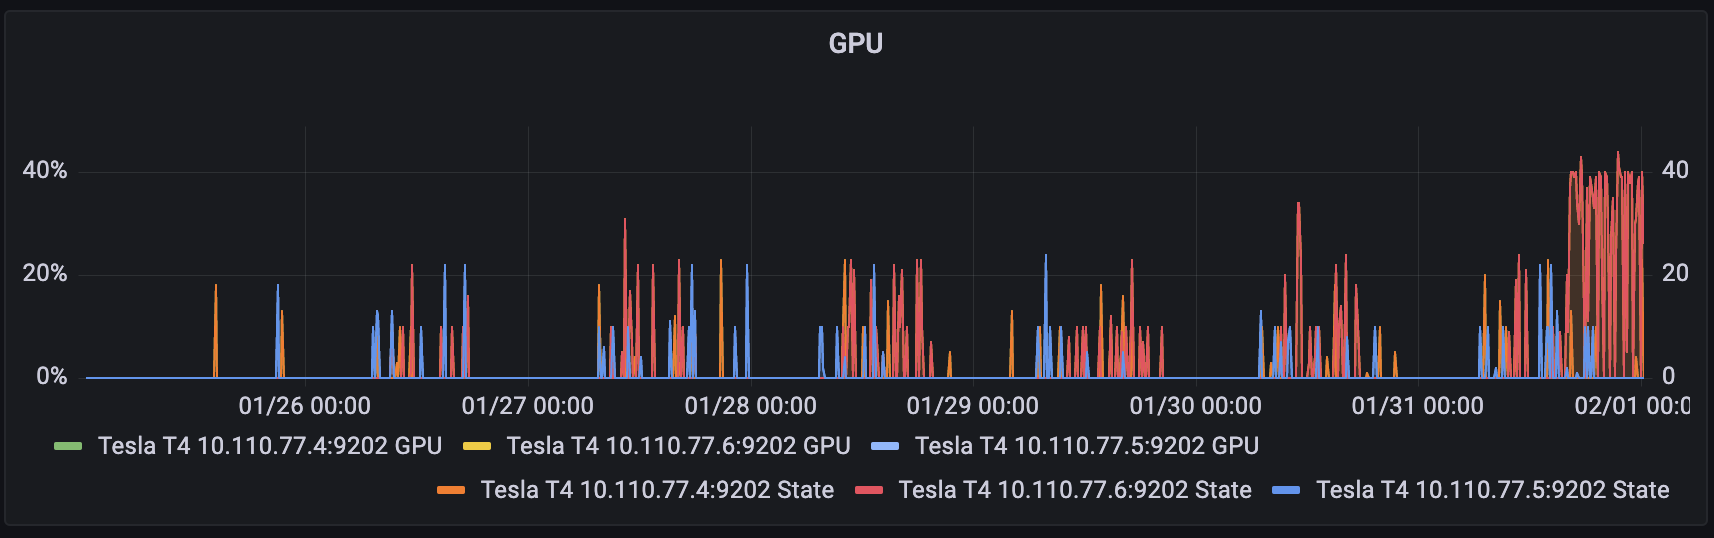
\includegraphics[width=1\textwidth]{figures/gpu_usage.png} 
    \caption{Mức độ sử dụng GPU trong 7 ngày gần nhất} % Creates caption underneath graph
    \label{fig:elk_01}
\end{figure}

Biểu đồ thể hiện mức độ sử dụng GPU được vẽ theo ngày (đương nhiên khoảng thời gian có thể được điều chính). Mức độ sát với thực tế khi GPU được sử dụng ít khi người dùng mới trở lại sau kì nghỉ Tết. Chúng ta hoàn toàn có thể đặt ngưỡng cảnh báo khi GPU bị cao tải (vượt ngưỡng 90\%)

\begin{figure}[H] % places figure environment here   
    \centering % Centers Graphic
    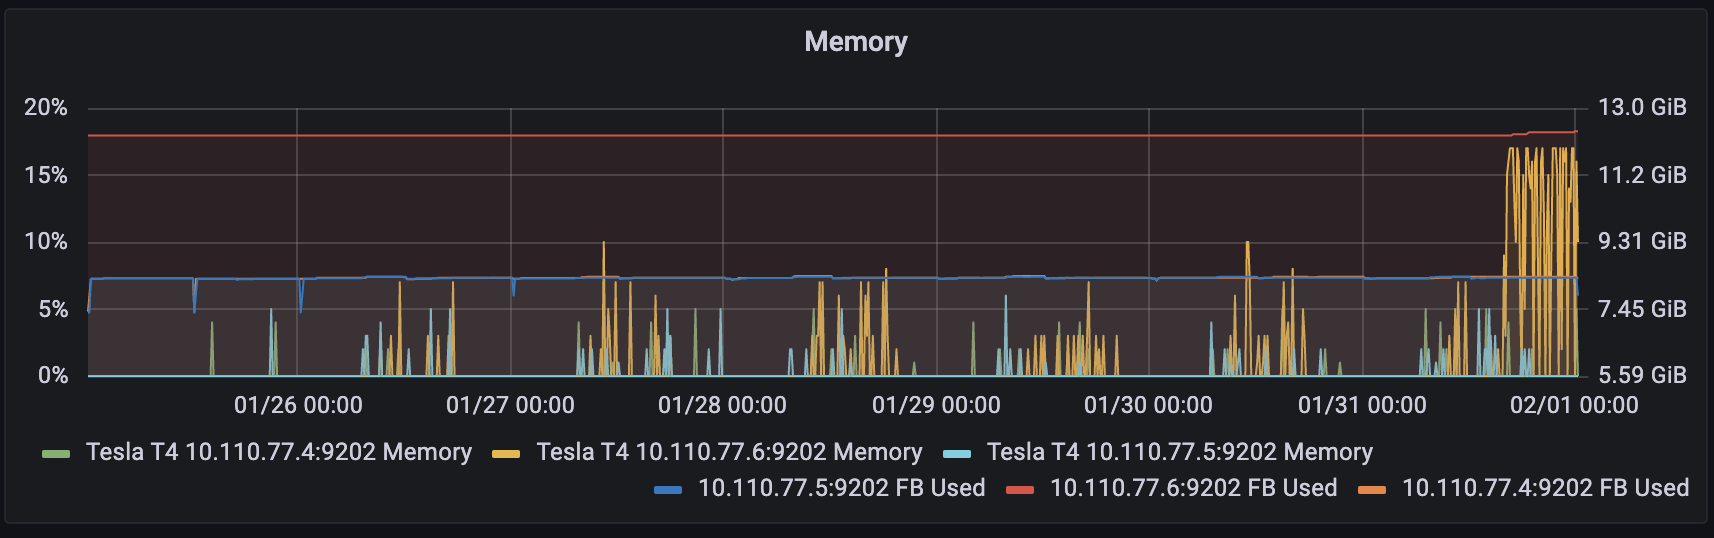
\includegraphics[width=1\textwidth]{figures/vram.png} 
    \caption{Mức độ sử dụng memory của GPU trong 7 ngày gần nhất} % Creates caption underneath graph
    \label{fig:elk_01}
\end{figure}

Tương ứng với mức độ sử dụng GPU ta cũng có biểu đồ về dung lượng VRAM được sử dụng. Ngưỡng cảnh báo tương tự cũng được áp dụng (90\%)

\begin{figure}[H] % places figure environment here   
    \centering % Centers Graphic
    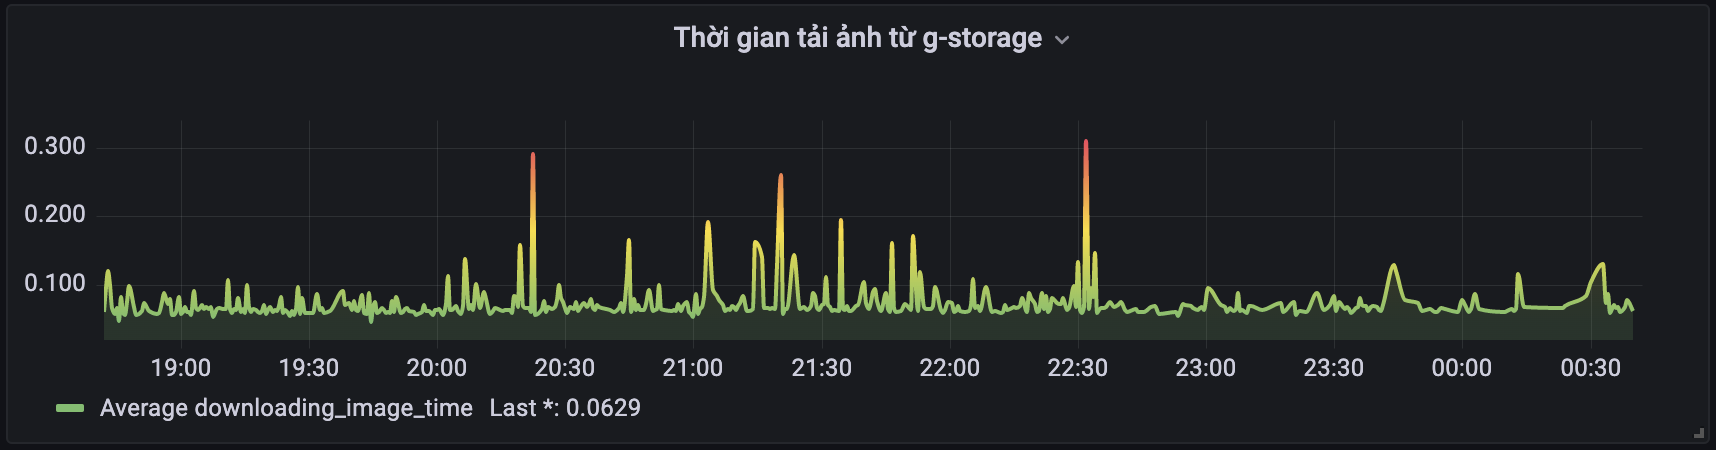
\includegraphics[width=1\textwidth]{figures/download_time.png} 
    \caption{Thời gian tải ảnh} % Creates caption underneath graph
    \label{fig:elk_01}
\end{figure}

Thời gian ứng dụng tải ảnh từ storage lưu trữ tập trung cũng được thể hiện bằng biểu đồ đường tương tự như những biểu đồ khác. 

Có thể nói Grafana được đội của tác giả sử dụng nhằm mục đính nắm tổng quan về hệ thống và đưa ra cảnh báo sớm. Các thông tin chi tiết hơn về ứng dụng hoặc một lỗi cụ thể sẽ được khám phá kĩ càng hơn với ELK Stack (sẽ được trình bày ở phần sau vủa bài).